\section{\large{\textbf{Junkers Ju 88}}}
%========================

\subsection{Początki}


\begin{frame}{\Huge{\textbf{Ju 88 - Początki}}}
	\begin{columns}[t]
		\column{0.39\textwidth} 
			\justifying

\textbf{Junkers Ju88} był jednym z dwóch projektów stworzonych w odpowiedzi na trzecie zapotrzebowanie RLM z 1935 roku na szybki samolot bombowy. Prace nad jego rozwojem rozpoczęto w styczniu 1936 roku, a projekt nosił oznaczenie EF59. Obok Ju88 powstawały również Henschel Hs127 i Messerschmitt Bf162. \\
W początkowej fazie rozwoju analizowano dwa główne projekty: Ju85 z podwójnym ogonem oraz Ju88 z pojedynczym ogonem. Choć początkowo preferowany był Ju85, ostatecznie zdecydowano się na bardziej nowoczesny projekt Ju88. Budowa prototypu rozpoczęła się w maju 1936, a pierwszy lot Ju88V1 miał miejsce 21 grudnia 1936. Zbudowano pięć prototypów, z których trzy miały projekt skrzydeł i kadłuba z Ju85.

		\column{0.61\textwidth}
			\begin{figure}
				\centering
				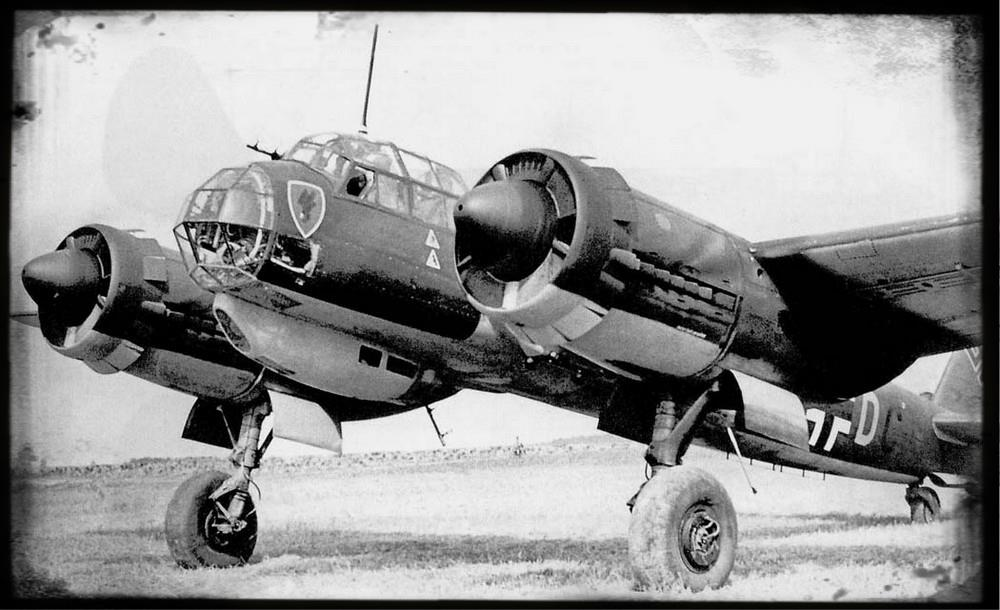
\includegraphics[scale=0.25]{images/ju88-01.jpg}
				\caption{\textit{Ju 88}}
			\end{figure}
	\end{columns}
\end{frame}


%~~~~~~~~~~~~~~~~~~~~~~~~~~~~~~~~~

\subsection{Rozwój}


\begin{frame}{\Huge{\textbf{Ju 88 - Rozwój}}}
	\begin{columns}[t]
		\column{0.67\textwidth} 
			\justifying
			
W 1937 roku zmieniono wymagania RLM, uwzględniając możliwość przystosowania Ju88 jako bombowca nurkującego. Prototyp Ju88V6, który spełniał nowe wymagania, wzbił się w powietrze 18 czerwca 1938 roku. Jesienią 1938 roku Ju88 został wybrany na standardowy bombowiec Luftwaffe, a plany produkcji zakładały maksymalnie 300 samolotów miesięcznie. Produkcja była rozproszona w różnych zakładach w Niemczech, a masowa produkcja ruszyła w 1940 roku. W ciągu sześciu lat zbudowano 15 000 Ju88, co czyniło go najczęściej produkowanym samolotem Junkersa. W trakcie produkcji wprowadzono 3000 zmian i opracowano wiele podtypów, co umożliwiło użycie Ju88 jako bombowca, myśliwca i samolotu rozpoznawczego. \\
Standardowa wersja bombowa to seria A, której produkcję rozpoczęto w 1938 roku, a masowa produkcja A4 rozpoczęła się w 1940. W sumie powstało 17 głównych podtypów Ju88A. Wersje B, C i G były rozwijane w celu zwiększenia zasięgu, prędkości i zastosowań bojowych, w tym jako myśliwce nocne. Pomimo wielu udoskonaleń, niektóre wersje, takie jak seria S nie spełniły oczekiwań w porównaniu do konkurencji. Ostatecznie Ju88 stał się wszechstronnym samolotem o różnych zastosowaniach podczas II wojny światowej.
			
		\column{0.33\textwidth}
			\begin{figure}
				\centering
				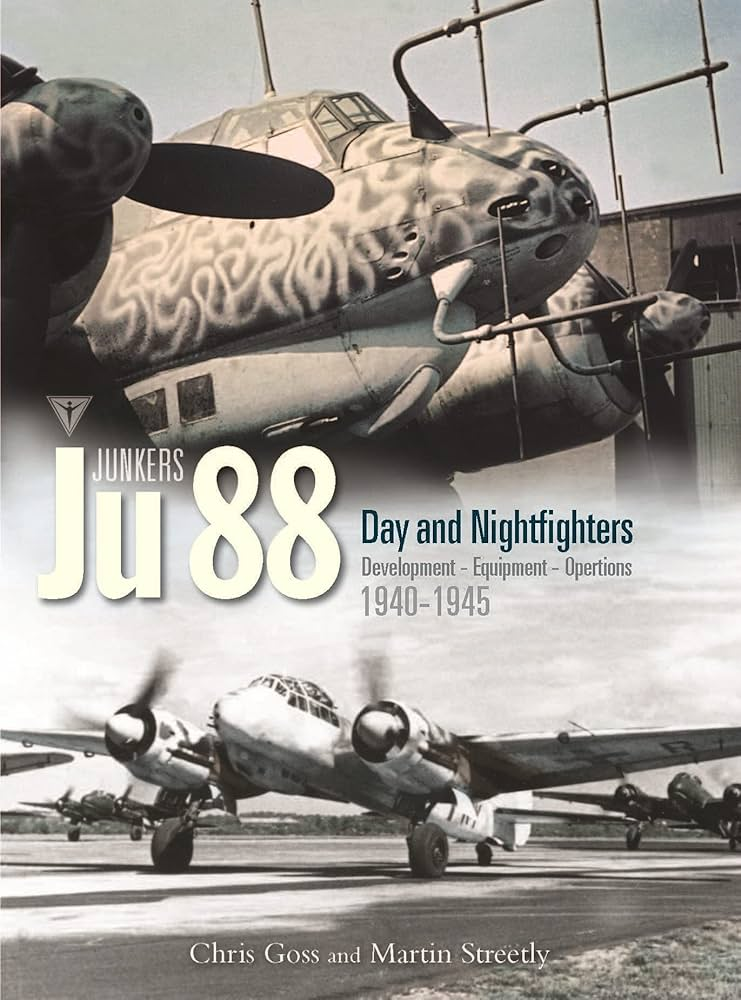
\includegraphics[scale=0.145]{images/ju88-02.jpg}
				\caption{\textit{Ju 88}}
			\end{figure}
	\end{columns}
\end{frame}


%~~~~~~~~~~~~~~~~~~~~~~~~~~~~~~~~~

\subsection{Warianty}


\begin{frame}[t]{\Huge{\textbf{Ju 88 - Warianty}}}
	\begin{columns}[t]
		\column{0.5\textwidth} 

{\large{\textbf{Wariant A}}}	\\~\
	\justifying

Produkcja masowa rozpoczęła się w 1940 roku z serią A4, a do końca II wojny światowej zaprojektowano około 17 głównych podtypów Ju88A, które były używane zarówno jako bombowce, jak i samoloty rozpoznawcze. W trakcie produkcji A4 wprowadzono różne modyfikacje, takie jak wzmocnienie podwozia, zwiększenie rozpiętości skrzydeł oraz zwiększenie masy operacyjnej. Model Ju88-A13 był wykorzystywany do ataków naziemnych i miał wzmocnioną osłonę, natomiast Ju88-A17 był wersją testową bombowca torpedowego.

		\column{0.5\textwidth}
		
{\large{\textbf{Wariant B}}}	\\~\
	\justifying

Seria B Ju88 została opracowana w 1940 roku w celu zwiększenia zasięgu, prędkości oraz ładunku militarnego. Zmodyfikowano przednią część samolotu, wprowadzając całkowicie przeszkloną kabinę. Zaprojektowano różne podtypy, w tym bombowce, samoloty rozpoznawcze i niszczyciele. Jednak zbudowano tylko kilka Ju88B, ponieważ RLM postanowiło kontynuować masową produkcję Ju88A, a modyfikacja zakładów produkcyjnych dla Ju88B okazała się zbyt skomplikowana. Zamiast Ju88B, RLM promowało Junkersa Ju288, który był nowym projektem opartym na Ju88. Gdy RLM zrozumiało, że rozwój Ju288 opóźni się, Ju88B stał się bazą dla ulepszonego Ju188, który miał być krokiem pośrednim do wprowadzenia Ju288.

	\end{columns}
\end{frame}

%----------------------------------------------

\begin{frame}[t]{\Huge{\textbf{Ju 88 - Warianty}}}
	\begin{columns}[t]
		\column{0.5\textwidth} 

{\large{\textbf{Wariant C}}}	\\~\
	\justifying

Seria C, znana również jako seria Z, była wersją niszczyciela i nocnego myśliwca Ju88, opracowaną od 1938 roku z modelu Ju88-V7, bazując na serii A. W przeciwieństwie do przeszklonej przedniej części A, seria C miała metalowy dziób oraz zdalnie sterowany karabin maszynowy na ogonie. Modele C2 i C3 były wykorzystywane jako "Jabos", wyposażone w uchwyty na bomby i karabiny maszynowe w przedniej części. Model C6 służył jako myśliwiec dzienny i nocny, był wyposażony w systemy radarowe oraz dodatkowe zdalnie sterowane karabiny maszynowe z tyłu kabiny.

		\column{0.5\textwidth}
		
{\large{\textbf{Wariant D}}}	\\~\
	\justifying

Seria D Ju88, produkowana od 1940 roku, była samolotem do strategicznego rozpoznania. Większość Ju88D to przebudowane modele Ju88A, w których usunięto hamulce nurkowe, a komora bombowa została wypełniona zbiornikami paliwa.

	\end{columns}
\end{frame}

%----------------------------------------------

\begin{frame}[t]{\Huge{\textbf{Ju 88 - Warianty}}}
	\begin{columns}[t]
		\column{0.5\textwidth} 

{\large{\textbf{Wariant G}}}	\\~\
	\justifying

Podczas II wojny światowej nocne myśliwce Ju88C stały się zbyt wolne, co doprowadziło do opracowania serii G jako nowej wersji nocnego myśliwca z mocniejszymi silnikami od 1942 roku. Nos serii G pochodził z modelu C6, natomiast tył kadłuba oparty był na konstrukcji Ju188. Skrzydła były klasycznymi skrzydłami z masowej produkcji A4. Ju88G stał się najbardziej udaną wersją nocnego myśliwca Luftwaffe od 1944 roku.

		\column{0.5\textwidth}
		
{\large{\textbf{Wariant H}}}	\\~\
	\justifying

Seria H została zapoczątkowana w 1943 roku jako samolot dalekiego zasięgu do zadań rozpoznawczych. Model H1 bazował na modelu D1, ale miał wydłużony kadłub o długości 17,88 m i zasięg 4700 km; wyprodukowano tylko dziesięć takich samolotów. Model H2 bazował na serii G, pierwotnie planowany jako G10. Zamówiono 20 samolotów H2, jednak nie jest jasne, czy którykolwiek został zbudowany.

	\end{columns}
\end{frame}

%----------------------------------------------

\begin{frame}[t]{\Huge{\textbf{Ju 88 - Warianty}}}
	\begin{columns}[t]
		\column{0.5\textwidth} 

{\large{\textbf{Wariant N i P}}}	\\~\
	\justifying

Serie N i P wyprodukowano w niewielkich ilościach. Zaprojektowano je jako samoloty do zwalczania czołgów na prośbę frontu wschodniego w 1942 roku, wyposażając w ciężkie działa przeciwpancerne. Problemy konstrukcyjne i testowe wynikały z dział, które powodowały pęknięcia strukturalne w dziobie i na śmigłach. W związku z tym zamontowano mniejsze działa BK3,7, używane już w modelu Ju87-G. Dodatkowe wzmocnienia sprawiły jednak, że modele P1/P2 były zbyt wolne, więc do modelu P3 dodano silniejszy silnik Jumo 211J, który ostatecznie trafił na front do prób. Część samolotów przekazano jednostkom myśliwskim na froncie zachodnim, ale z powodu ciężkich dział ich osiągi były słabe. 

		\column{0.5\textwidth}
		
{\large{\textbf{Wariant S}}}	\\~\
	\justifying

Serię S rozwijano od 1942 roku, gdy RLM zażądało poprawy prędkości bombowców Ju88. Bazując na serii A4, seria S otrzymała nową, aerodynamiczną, przeszkloną przednią część kadłuba. Prototyp Ju88S porównano z modelami Me410, Arado Ar240 i Heinkel Ke219 w Rechlin w 1943 roku, jednak nie osiągnął on wydajności konkurencyjnych modeli. Mimo to około 40 egzemplarzy Ju88S przebudowano z Ju88-A4.

	\end{columns}
\end{frame}

%----------------------------------------------

\begin{frame}[t]{\Huge{\textbf{Ju 88 - Warianty}}}
	\begin{columns}[t]
		\column{0.5\textwidth} 

{\large{\textbf{Wariant T}}}	\\~\
	\justifying

Seria T była wersją rozpoznawczą serii S. Produkcja na małą skalę rozpoczęła się w zakładach Henschel w Schönefeld jesienią 1944 roku, ale wkrótce została przerwana na rzecz modelu Messerschmitt Me410.

		\column{0.5\textwidth}
	\end{columns}
\end{frame}